\documentclass[english,12pt,a4paper]{book}
\usepackage[T1]{fontenc}
\usepackage[inner=3cm, outer=2cm, top=2.5cm, bottom=2.5cm]{geometry}
\usepackage{amssymb, graphicx, amsfonts, amsthm, tikz, listings, indentfirst, multirow, caption, pgfplots, newpx}
\usepackage[table,xcdraw]{xcolor}
\usepackage[bahasa]{babel}
\usetikzlibrary{shapes.geometric, arrows, shapes.symbols} 
\usepackage[toc,page]{appendix}
\usepackage[style=apa, backend=biber]{biblatex} 

\renewcommand{\bibname}{Daftar Pustaka}

\begin{document}
	\begin{titlepage}
		\centering
		% TODO: \usepackage{graphicx} required
		
\includegraphics[width=0.15\textwidth]{logounesa.png}\\[2ex]
		{\Large \textsc{Laporan Tugas Akhir}}\\[2ex]
		{\LARGE\bfseries Komputasi Matematika}\\[8ex]
		{\large Judul}\\[7cm]
		\textbf{Kelompok X - 2023Y}\\[2ex]
			Nama Anggota 1 - 23030214XXX\\
			Nama Anggota 2 - 23030214XXX\\
			Nama Anggota 3 - 23030214XXX\\
			dst
		\vfill
		Dosen Pengampu:\par
		Dimas Avian \textsc{Maulana}, M.Si.\\
		% Dr. Rahmawati Erma Standsyah, M.Si.\\ (untuk 2023B)
	
		\vfill
		{\large\textsc{Kementerian Pendidikan Tinggi, Sains, dan Teknologi} \par}
		{\large\textsc{Universitas Negeri Surabaya} \par}
		{\large\textsc{Fakultas Matematika dan Ilmu Pengetahuan Alam} \par}
		{\large\textsc{Program Studi S1 Matematika} \par}
		\vspace{1cm}
		% Bottom of the page
		{\large \today\par}
	\end{titlepage}
	
	\tableofcontents
	
\chapter{Pendahuluan}
\section{Latar Belakang}
Awali dengan gambaran umum tentang topik tugas akhir. Paparkan fenomena atau permasalahan spesifik yang ingin diangkat dalam tugas akhir. Sebutkan beberapa penelitian terdahulu yang relevan dengan topik penelitian. Setelah membahas konteks dan permasalahan, jelaskan fokus penelitian secara ringkas. Nyatakan variabel-variabel yang akan diteliti dan bagaimana hubungan antar variabel tersebut. Sampaikan juga metode penelitian yang akan digunakan. Akhiri latar belakang dengan menyebutkan judul penelitian secara lengkap.
\section{Rumusan Masalah}
Berdasarkan latar belakang yang telah diuraikan, rumusan masalah dalam penelitian ini adalah:
\begin{enumerate}
	\item Rumusan masalah 1, diawali dengan kata tanya seperti "Bagaimana", "Apa", "Apakah", dsb.
	\item Rumusan masalah 2, diawali dengan kata tanya
	\item Rumusan masalah 3 (jika ada)
\end{enumerate}
\section{Tujuan}
Tujuan dari penelitian ini adalah:
\begin{enumerate}
	\item Tujuan 1, untuk menjawab rumusan masalah 1
	\item Tujuan 2, untuk menjawab rumusan masalah 2
	\item Tujuan 3 (jika ada)
\end{enumerate}
Uraikan tujuan dari topik yang diangkat
\section{Manfaat}
Penelitian ini diharapkan dapat memberikan manfaat sebagai berikut:
\begin{enumerate}
	\item Manfaat Teoritis:
	\begin{enumerate}
		\item Manfaat penelitian untuk pengembangan ilmu pengetahuan di bidang studi yang relevan
		\item Manfaat penelitian sebagai referensi untuk penelitian selanjutnya
	\end{enumerate}
	\item Manfaat Praktis:
\begin{enumerate}
	\item Manfaat penelitian bagi ()sebutkan pihak yang mendapatkan manfaat praktis, misal: perusahaan, instansi, masyarakat, dll.)
	\item Manfaat penelitian sebagai bahan pertimbangan dalam pengambilan keputusan terkait ()sebutkan bidang/isu yang relevan)
\end{enumerate}
\end{enumerate}

\chapter{Tinjauan Pustaka}
Uraikan tinjau pustaka yang relevan dengan topik penelitian. Misalkan judul tugas akhir adalah Penerapan Metode \textit{Analytical Hierarchy Process} dalam Penentuan Makanan Favorit di Alam Semesta. Maka subbab yang harus ditulis adalah:
\section{Metode AHP}
Uraikan tentang Metode AHP
\section{Makanan Favorit}
Uraikan dan jelaskan bagaimana suatu makanan bisa menjadi makanan favorit

\chapter{Metode Penelitian} 
\section{Populasi dan Sampel Penelitian}
\begin{enumerate}
	\item Populasi: Keseluruhan objek atau subjek yang memiliki karakteristik tertentu yang ingin diteliti. Contoh: seluruh mahasiswa Universitas Indonesia, seluruh karyawan di sebuah perusahaan, seluruh penduduk di suatu kota.
	\item Sampel: Bagian dari populasi yang dipilih untuk diteliti. Sampel harus representatif, artinya dapat mewakili karakteristik populasi secara keseluruhan.
\end{enumerate}
\section{Variabel Penelitian}
Variabel adalah sesuatu yang dapat diukur atau diamati dan memiliki nilai yang bervariasi.
\begin{enumerate}
	\item Variabel independen (bebas): Variabel yang diduga menjadi penyebab atau memengaruhi variabel lain.
	\item Variabel dependen (terikat): Variabel yang diduga dipengaruhi oleh variabel independen.
	\item Variabel moderator: Variabel yang dapat memperkuat atau memperlemah hubungan antara variabel independen dan dependen.
	\item Variabel kontrol: Variabel yang dijaga agar tetap konstan untuk menghindari pengaruhnya terhadap variabel lain.
\end{enumerate}
\section{Instrumen Penelitian}
Instrumen penelitian adalah alat yang digunakan untuk mengumpulkan data dalam penelitian. Contoh instrumen penelitian:
\begin{enumerate}
	\item Kuesioner: Serangkaian pertanyaan tertulis yang diberikan kepada responden untuk dijawab.
	\item Wawancara: Proses tanya jawab secara langsung antara peneliti dan responden.
	\item Observasi: Pengamatan langsung terhadap suatu fenomena atau perilaku.
	\item Tes: Alat ukur untuk mengukur kemampuan, pengetahuan, atau karakteristik tertentu.
	\item Dokumentasi: Pengumpulan data dari dokumen-dokumen seperti arsip, laporan, catatan, dll.
\end{enumerate}
\section{Teknik Pengumpulan Data}
Cara yang digunakan untuk memperoleh data dalam penelitian. Beberapa teknik pengumpulan data antara lain:
\begin{enumerate}
	\item Survey: Pengumpulan data dari sejumlah besar responden melalui kuesioner atau wawancara.
	\item Eksperimen: Melakukan percobaan untuk menguji pengaruh suatu variabel terhadap variabel lain.
	\item Studi kasus: Penelitian mendalam terhadap suatu kasus atau fenomena tertentu.
\end{enumerate}
\begin{table}[h!]
	\centering
	\caption{Pengelompokan jenis roti di Lyly Bakery Lamongan}
	\begin{tabular}{|l|l|l|}
		\hline
		No                    & Pengelompokan                       &                               \\ \hline
		\multirow{10}{*}{1.}  & \multirow{10}{*}{Donat}             & Donat strawberry marble      \\ \cline{3-3} 
		&                                     & Donat chocolate peanut       \\ \cline{3-3} 
		&                                     & Donat chocolate marble       \\ \cline{3-3} 
		&                                     & Donat white choco almond     \\ \cline{3-3} 
		&                                     & Donut icing sugar            \\ \cline{3-3} 
		&                                     & Donat misis mix              \\ \cline{3-3} 
		&                                     & Donat misis coklat           \\ \cline{3-3} 
		&                                     & Conat chicken                \\ \cline{3-3} 
		&                                     & Donat keju                   \\ \cline{3-3} 
		&                                     & Donat merah putih            \\ \hline
	\end{tabular}
\end{table}
\section{Teknik Analisis Data}
Cara yang digunakan untuk mengolah dan menginterpretasi data yang telah dikumpulkan.
\begin{enumerate}
	\item Analisis kuantitatif: Analisis data yang menggunakan angka-angka dan statistik. Contoh: uji-t, analisis regresi, analisis varians.
	\item Analisis kualitatif: Analisis data yang berupa kata-kata, gambar, atau objek. Contoh: analisis isi, analisis naratif, grounded theory.
\end{enumerate}
\section{Pelaksanaan Penelitian}
Kegiatan penelitian ini akan mengikuti jadwal yang telah disusun pada~\ref{tab:kegiatan} berikut.

\begin{center}
	\tikzstyle{startstop} = [rectangle, rounded corners=0.5cm, minimum width=2.5cm, minimum height=1cm, text centered, draw=black]
	\tikzstyle{io} = [trapezium, trapezium stretches=true, trapezium left angle=70,  trapezium right angle=110, minimum height=1cm, text centered, draw=black]
	\tikzstyle{process} = [rectangle, minimum width=2cm, minimum height=1cm, text centered, draw=black]
	\tikzstyle{decision} = [diamond, minimum height=1cm, aspect=2.5, text centered, draw=black]
	\tikzset{connector/.style={shape=signal, draw, signal to=south,text width=1cm,text height=0.5cm, align=center},
	}
	\tikzstyle{arrow} = [ultra thick,->,>=stealth]
	
	\begin{tikzpicture}[node distance=2cm]
		\node (start) [startstop] {Mulai};
		\node (in) [io, below of=start] {Data Saham};
		\node (pro2) [decision, below of=in] {Input Parameter};
		\node (pro3) [process, below of=pro2] {Hitung nilai $dt, u, d, p, v_{es}$ dan $S_{ij}$};
		\node (pro4) [process, below of=pro3] {Menghitung harga opsi saat jatuh tempo};
		\node (pro5) [process, below of=pro4] {Melakukan hitung mundur seperti metode Binomial untuk memperoleh $f_{0,0}$};
		\node (con) [connector, below of=pro5] {A};
		\node (stop) [startstop, below of=con] {Selesai};
		
		\draw [arrow] (start) -- (in);
		\draw [arrow] (in) -- (pro2);
		\draw [arrow] (pro2) -- (pro3);
		\draw [arrow] (pro3) -- (pro4);
		\draw [arrow] (pro4) -- (pro5);
		\draw [arrow] (pro5) -- (con);
		\draw [arrow] (con) -- (stop);		
	\end{tikzpicture}
	\captionof{figure}{Alur penelitian}
\end{center}

\begin{figure}[h!]
	\centering
	\begin{tikzpicture}
		\begin{axis}[
			ybar,
			ymin=-1.5,
			ymax=1.5,
			symbolic x coords={$\alpha$,$\beta$,$d$,$\gamma$,$\kappa$,$\mu$,$\omega$,$\phi$},
			xtick=data,
			nodes near coords,
			nodes near coords align={vertical},
			nodes near coords style={font=\footnotesize},
			grid=major,
			]
			\addplot[
			color=black!70,
			fill=black!30,
			] coordinates {
				($\alpha$,1)
				($\beta$,0.175)
				($d$,-0.061)
				($\gamma$,-0.87)
				($\kappa$, -0.15)
				($\mu$, 0.53)
				($\omega$, 0.34)
				($\phi$, -0.97)
			};
		\end{axis}
	\end{tikzpicture}
	\caption{Indeks sensitivitas}
\end{figure}

\chapter{Hasil dan Pembahasan}
Tampilkan hasil \textit{running} program disini
\begin{figure}
	\centering
	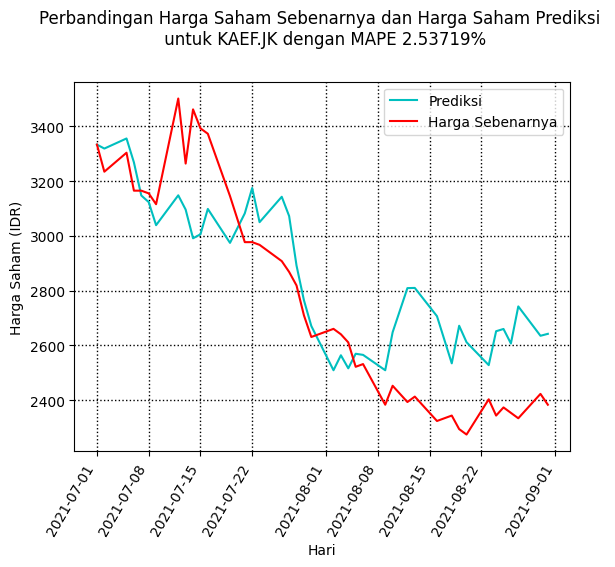
\includegraphics[width=\linewidth]{KAEF}
	\caption{Hasil running program dengan input xxx}
	\label{fig:kaef}
\end{figure}

\chapter{Kesimpulan dan Saran}
\section{Kesimpulan}
Kesimpulan adalah bagian penting dalam tugas akhir yang merangkum inti dari seluruh penelitian. Bagian ini berisi pernyataan ringkas dan padat yang menjawab rumusan masalah dan tujuan penelitian. Berikut adalah hal-hal yang perlu diperhatikan dalam menulis kesimpulan:
\begin{enumerate}
	\item Ringkasan inti: Fokus pada poin-poin penting yang ditemukan dalam penelitian. Hindari mengulang isi pembahasan secara detail.
	\item Jawaban atas rumusan masalah: Pastikan setiap rumusan masalah terjawab dengan jelas dan lugas.
	\item Keterkaitan dengan tujuan: Tunjukkan bagaimana hasil penelitian mencapai tujuan yang telah ditetapkan.
	\item Berdasarkan data: Semua kesimpulan harus didasarkan pada data dan analisis yang telah dilakukan, bukan opini pribadi.
	\item Bahasa yang ringkas dan padat: Gunakan bahasa yang mudah dipahami dan hindari kalimat yang bertele-tele.
\end{enumerate}
Contoh Kesimpulan:\\
Berdasarkan hasil penelitian dan analisis data yang telah dilakukan, dapat disimpulkan bahwa: ...

\section{Saran}
Saran adalah bagian yang berisi rekomendasi atau masukan dari peneliti berdasarkan hasil penelitian. Saran ditujukan kepada pihak-pihak terkait agar dapat memanfaatkan hasil penelitian atau melakukan perbaikan di masa mendatang. Berikut adalah hal-hal yang perlu diperhatikan dalam menulis saran:
\begin{enumerate}
	\item Relevan dengan hasil penelitian: Saran harus berkaitan erat dengan kesimpulan dan temuan penelitian.
	\item Bersifat konstruktif dan solutif: Berikan saran yang membangun dan memberikan solusi atas permasalahan yang diangkat.
	\item Spesifik dan terarah: Saran harus jelas, spesifik, dan ditujukan kepada pihak-pihak tertentu.
	\item Mempertimbangkan keterbatasan: Saran perlu mempertimbangkan keterbatasan penelitian dan kendala yang mungkin dihadapi.
\end{enumerate}

\begin{thebibliography}{9} 
	\bibitem{Azuela} Mariano Azuela, \textit{The Underdogs: A Novel of the Mexican Revolution}, trans. Beth Jorgensen (New York: The Modern Library, 2002). 
\end{thebibliography}

\appendix
	\chapter{\textit{Source Code}}
	Tuliskan \textit{source code} disini. Berikut adalah contoh \textit{source code}:
	\lstinputlisting[language=python, basicstyle=\ttfamily, numbers=left]{PCA.py} %ganti epidemiology.py dengan file Anda
\end{document}

